\documentclass[12pt, titlepage]{article}

\usepackage{xcolor} % for different colour comments
\usepackage{tabto}
\usepackage{mdframed}
\usepackage{xkeyval}
\usepackage{tabularx}
\usepackage{booktabs}
\usepackage{hyperref}
\hypersetup{
    colorlinks,
    citecolor=black,
    filecolor=black,
    linkcolor=red,
    urlcolor=blue
}
\usepackage[singlelinecheck=off, skip=2pt, labelfont=bf]{caption}
\usepackage{titlesec}
\usepackage{graphicx}
\graphicspath{ {image/} }



%% the following adds another section level by redefining the paragraph
%% source:  http://tex.stackexchange.com/questions/60209/how-to-add-an-extra-level-of-sections-with-headings-below-subsubsection
\setcounter{secnumdepth}{4}

\titleformat{\paragraph}
{\normalfont\normalsize\bfseries}{\theparagraph}{1em}{}
\titlespacing*{\paragraph}
{0pt}{3.25ex plus 1ex minus .2ex}{1.5ex plus .2ex}



%% used for counting in event list
\newcounter{EventList}
\newcommand{\printEvent}{
    \stepcounter{EventList}
    \arabic{EventList}.
}

%% used for counting in phase list
\newcounter{PhaseList}
\newcommand{\printPhase}{
    \stepcounter{PhaseList}
    \arabic{PhaseList}.
}



%% Comments
\newif\ifcomments\commentstrue

\ifcomments
\newcommand{\authornote}[3]{\textcolor{#1}{[#3 ---#2]}}
\newcommand{\todo}[1]{\textcolor{red}{[TODO: #1]}}
\else
\newcommand{\authornote}[3]{}
\newcommand{\todo}[1]{}
\fi

\newcommand{\wss}[1]{\authornote{magenta}{SS}{#1}}
\newcommand{\ds}[1]{\authornote{blue}{DS}{#1}}



%% The following are used for pretty printing of events and requirements
\makeatletter

\define@cmdkey      [SRS] {req}     {use}       {}
\define@cmdkey      [SRS] {req}     {desc}      {}
\define@cmdkey      [SRS] {req}     {rationale} {}
\define@cmdkey      [SRS] {req}     {orig}      {}
\define@cmdkey      [SRS] {req}     {fit}       {}
\define@cmdkey      [SRS] {req}     {sat}       {}
\define@cmdkey      [SRS] {req}     {dissat}    {}
\define@cmdkey      [SRS] {req}     {priority}  {}
\define@cmdkey      [SRS] {req}     {conf}      {}
\define@cmdkey      [SRS] {req}     {supp}      {}
\define@cmdkey      [SRS] {req}     {hist}      {}

\define@cmdkey      [SRS] {event} {name}      {}
\define@cmdkey      [SRS] {event} {trigger}   {}
\define@cmdkey      [SRS] {event} {precond}   {}
\define@cmdkey      [SRS] {event} {postcond}  {}

\newcounter{EventNum}
\newcommand{\event}[1]{
\setkeys[SRS]{event}{#1}
\refstepcounter{EventNum}
\begin{mdframed}
\noindent {\bf Use Case \#:} \arabic{EventNum}\\[\baselineskip]
\begin{tabularx}{\textwidth}{@{}p{3cm}X@{}}
{\bf Name:} & \cmdSRS@event@name\\
{\bf Trigger:} & \cmdSRS@event@trigger\\
{\bf Precondition:} & \cmdSRS@event@precond\\
{\bf Postcondition:} & \cmdSRS@event@postcond
\end{tabularx}
\end{mdframed}
}


\newcounter{ReqNum}
\newcommand{\req}[1]{
\setkeys[SRS]{req}{#1}
\stepcounter{ReqNum}
\begin{mdframed}
\noindent {\bf Requirement \#:} \arabic{ReqNum} \tabto{4.3cm} {\bf Requirement Type:} \arabic{section}.\arabic{subsection} \tabto{9.8cm} {\bf Use Case:} \cmdSRS@req@use\\[\baselineskip]
\begin{tabularx}{\textwidth}{@{}p{3cm}X@{}}
{\bf Description:} & \cmdSRS@req@desc\\
{\bf Rationale:} & \cmdSRS@req@rationale\\
{\bf Fit Criterion:} & \cmdSRS@req@fit\\[\baselineskip]
\end{tabularx}
\begin{tabularx}{0.5\textwidth}{@{}p{4cm}X@{}}
{\bf Cust. Satisfaction:} & \cmdSRS@req@sat \\
{\bf Priority:} & \cmdSRS@req@priority \\[\baselineskip]
\end{tabularx}
\begin{tabularx}{0.5\textwidth}{@{}p{4.5cm}X@{}}
{\bf Cust. Dissatisfaction:} & \cmdSRS@req@dissat\\
{\bf Conflicts:} & \cmdSRS@req@conf\\[\baselineskip]
\end{tabularx}
\begin{tabularx}{\textwidth}{@{}p{5cm}X@{}}
{\bf Supporting Materials:} & \cmdSRS@req@supp\\
{\bf History:} & \cmdSRS@req@hist
\end{tabularx}
\end{mdframed}}

\makeatother


\begin{document}

\title{\bf Physics-Based Chipmunk2D Game\\[\baselineskip]\Large Software Requirements Specification\\[2\baselineskip] \large Based on the Volere Template}
\author{Steven Palmer\\Emaad Fazal\\Chao Ye}
\date{\today}
	
\maketitle

\pagenumbering{roman}
\tableofcontents
\listoftables
\listoffigures

\begin{table}[bp]
\caption*{\bf Revision History}
\begin{tabularx}{\textwidth}{p{3cm}p{2cm}X}
\toprule {\bf Date} & {\bf Version} & {\bf Notes}\\
\midrule
October 7, 2015 & 1.0 & Created document\\
October 7, 2015 & 1.1 & Major edits in progress\\
October 8, 2015 & 1.2 & Major event and reqs additions\\
October 9, 2015 & 1.3 & Final version for rev 0 hand-in\\
\bottomrule
\end{tabularx}
\end{table}

\newpage

\pagenumbering{arabic}
\section{Project Drivers}
\subsection{The Purpose of the Project}
The purpose of this project is to produce a game that will be used as a demonstration for students in a third year software engineering game design course at McMaster University.  The game will incorporate the \href{https://chipmunk-physics.net/}{Chipmunk2D} physics library and highlight its capabilities.
\subsection{The Stakeholders}
\subsubsection{The Client}
The client for this project is \href{http://www.cas.mcmaster.ca/~smiths/}{Dr.~Spencer Smith} of the Computing and Software department at McMaster University.
\subsubsection{The Customers}
The customers for this project are students who will take the game design course in the future.
\subsubsection{Other Stakeholders}
Other stakeholders include future instructors of the game design course or other similar courses.

\newpage
\section{Project Description}
\subsection{Game Overview}
For this project an action-role playing type game will be created.  It will consist of a game world within which a user-controlled hero makes progress by defeating enemies.  The subsections that follow provide a more detailed explanation of the game.

\subsubsection{The Game World}
The game world is the virtual environment in which all gameplay takes place.  This environment is made up of platforms which the hero and enemies are permitted to stand on, as well as obstacles which limit the possible movements of the hero throughout the game and hazards which can cause damage or unwanted effects to both the hero and enemies.


\subsubsection{The Hero}
The hero is the protagonist of the game, and is controlled by the user.

\paragraph{Movement}
The hero is able to move left or right, and to jump, in order to progress through the game.  The hero can interact with several objects in the game.  These objects include enemies, obstacles, and hazards.  When the hero comes into contact with an object an event is triggered.  Depending on the type of object, these events include:

\begin{enumerate}
  \item If the object is an enemy the hero will lose health and be knocked back from the enemy.
  \item If the object is an obstacle the hero will be stopped and unable to pass.
  \item If the object is an environmental hazard the hero may lose health and be knocked back depending on the type of hazard.
\end{enumerate}

\paragraph{Attack}
The hero is able to attack enemies using weapons.  Weapons are defined by their fire rate, power, bullet travel distance, and ammo capacity. These characteristics provide certain weapons with advantages over others depending on the type of enemy being fought.

Weapons are divided into three classes: pistols, shotguns, and rifles. Each class of weapons has its own benefits and faults. Pistols are weak in terms of their power but have infinite ammo and are always available for the player to use.  They provide a way for the user to conserve ammo in dire situations.  They also provide a last ditch effort when no ammo is available for the other two weapon classes.  Shotguns are very powerful but have very short range and limited ammo capacity. They provide an efficient way to deal with a large amount of enemies at once.  Rifles provide good range to hit enemies from a distance, and tend to be more powerful than pistols but weaker than shotguns.

\paragraph{Score}
As the hero defeats enemies, his or her score is increased.  The amount by which the hero's score is increased depends on how powerful the defeated enemy was. Increasing the hero's score offers access to more powerful weapons and allows navigation into deeper areas of the game world where more powerful enemies lurk.




\subsubsection{The Enemies}
Enemies are found throughout the game and are programmed to attack the hero with the goal of defeating him or her.  When an enemy is encountered during the game, combat will ensue if the hero gets within a certain range.  The user may attempt to avoid the enemy or to flee if he or she has come close enough to trigger combat.

\paragraph{Movement}
Enemy movement is controlled by the game AI.  When the hero is within a certain range of an enemy, the game AI will respond by moving the enemy in a manner defined in the game code.

\paragraph{Attack}
Enemy attacks are also controlled by the game AI.  When the hero is within a certain range of an enemy, the game AI will respond by attacking in a manner defined in the game code.  Unlike the hero, the enemies do not use weapons, but instead have inherent attacks which vary by enemy type.



\subsection{Mandated Constraints}

The project is subject to the following mandated constraints:

\begin{enumerate}
  \item The game must make significant use of the Chipmunk2D physics library.
  \item The game must support all major PC operating systems.
  \item Project milestones must be completed by the dates given in the CS 4ZP6 syllabus.
  \item The project must be fully completed by April 1, 2015.
\end{enumerate}

\subsection{Naming Conventions and Terminology}
The terminology used in this project is given in \hyperref[tab:terminology]{Table~\ref*{tab:terminology}}.
\begin{table}[h]
\caption{List of terminology} \label{tab:terminology}
\begin{tabularx}{\textwidth}{p{3cm}X}
\toprule {\bf Term} & {\bf Definition}\\
\midrule
AI & Artificial intelligence\\
Bounds & The boundaries inside which game play occurs\\
Enemy & Hostile character; attacks hero if hero is in range\\
Hazard & An environmental object that causes negative effects to the hero\\
Hero & The main character of the game controlled by the user\\
Hit Points & The amount of damage the hero or an enemy can take before being defeated\\
Obstacle & A barrier that the hero cannot cross\\
Score & Measure of progress in the game\\
User & Player of the game\\
\bottomrule
\end{tabularx}
\end{table}

\newpage
\section{Functional Requirements}
\subsection{The Scope of the Work and the Product}

\subsubsection{The Context of the Work}
A context diagram of the the work is given in \hyperref[fig:context]{Figure~\ref*{fig:context}}.

\begin{figure}[hb]
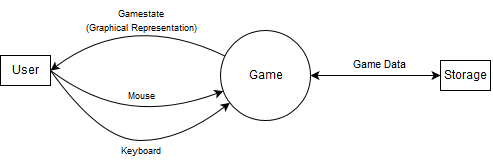
\includegraphics[width=\textwidth]{context}
\caption{Context diagram of the work} \label{fig:context}
\end{figure}


\subsubsection{Work Partitioning}
The flow diagram in \hyperref[fig:gameflow]{Figure~\ref*{fig:gameflow}} gives a rough representation of the operation of the envisioned game.  The user interfaces include a main menu as well as an in-game menu, and an in-game interface in which all game play takes place.  The events are listed in \hyperref[tab:events]{Table~\ref*{tab:events}}.
\begin{figure}
\includegraphics[width=\textwidth]{game_flow}
\caption[Flow diagram of the game]{Flow diagram of the game.  Ovals represent user interfaces and rectangles represent events.} \label{fig:gameflow}
\end{figure}

\begin{table}
\caption{List of events} \label{tab:events}
\begin{tabularx}{\textwidth}{p{0.5cm}>{\raggedright}p{3cm}>{\raggedright}p{3.5cm}>{\raggedright\arraybackslash}X}
\toprule & {\bf Event Name} & {\bf Inputs/Outputs} & {\bf Summary}\\
\midrule
\printEvent & New Game & Mouse (in) & A new game is started\\
\printEvent & Load Game & Game File (in) & A game file is loaded\\
\printEvent & Save Game & Game File (out) & A saved game file is created\\
\printEvent & Exit to Main Menu & Mouse (in) & Exit from current game to main menu\\
\printEvent & Move Hero & Keyboard (in) Gamestate (out) & The hero moves through the game world\\
\printEvent & Hero Attack & Keyboard (in) Gamestate (out) & The hero attacks an enemy\\
\printEvent & Change Weapon & Keyboard (in) Gamestate (out) & The hero's current weapon is changed\\
\printEvent & Hero Contacts Hazard & Gamestate (out) & The hero comes into contact with a hazard\\
\printEvent & Hero Takes Damage & Gamestate (out) & The hero loses hit points\\
\printEvent & Hero is Defeated & Gamestate (out) & The hero's hit points reach zero and the game ends\\
\printEvent & Move Enemy & Gamestate (out) & An enemy moves through the game world\\
\printEvent & Enemy Attack & Gamestate (out) & An enemy attacks the hero\\
\printEvent & Enemy Contacts Hazard & Gamestate (out)  & An enemy comes into contact with a hazard\\
\printEvent & Enemy Takes Damage & Gamestate (out) & An enemy loses hit points\\
\printEvent & Enemy is Defeated & Gamestate (out) & An enemy's hit points reach zero\\
\printEvent & Open In-Game Menu & Keyboard (in) & The in-game menu is opened\\
\printEvent & Close In-Game Menu & Mouse (in) & The in-game menu is closed\\
\printEvent & Exit Game & Mouse (in) & The game application is terminated\\
\bottomrule 
\end{tabularx}
\end{table}

\subsubsection{Individual Product Use Cases}

Due to the nature of the project, the product use cases are essentially equivalent to the events identified in the work partitioning.  

\event{
    name = New Game,
    trigger = The user selects to start a new game,
    precond = The main menu is open,
    postcond = A new game commences
} \label{event:newgame}

\event{
    name = Load Game,
    trigger = The user selects to load a game,
    precond = The main menu or in-game menu is open,
    postcond = A saved game state is loaded and the game commences from that point
} \label{event:loadgame}

\event{
    name = Save Game,
    trigger = The user selects to save a game,
    precond = The in-game menu is open,
    postcond = A saved game state is created
} \label{event:savegame}

\event{
    name = Exit to Main Menu,
    trigger = The user selects exit game,
    precond = The in-game menu is open,
    postcond = Current game is ended and main menu is opened
} \label{event:exittomain}

\event{
    name = Move Hero,
    trigger = Inputs from user related to controlling the hero movement,
    precond = In-game,
    postcond = Hero moves according to input
} \label{event:movehero}

\event{
    name = Hero Attack,
    trigger = Inputs from user related to hero attack,
    precond = In-game,
    postcond = Hero's currently selected attack is activated
}  \label{event:heroattack}

\event{
    name = Change Weapon,
    trigger = Input from user related to hero weapon (hotkeys),
    precond = In-game,
    postcond = Hero's currently active weapon is switched according to input
} \label{event:changeweapon}

\event{
    name = Hero Contacts Hazard,
    trigger = Hero comes into contact with hazard,
    precond = In-game,
    postcond = Hero is affected by the hazard
} \label{event:herohazard}

\event{
    name = Hero Takes Damage,
    trigger = Enemy contacts hazard or enemy is attacked by hero,
    precond = In-game,
    postcond = Enemy hit points are reduced
} \label{event:herodamaged}

\event{
    name = Hero is Defeated,
    trigger = Hero hit points reach zero,
    precond = In-game,
    postcond = Current game is ended and main menu is opened
} \label{event:herodefeated}

\event{
    name = Move Enemy,
    trigger = Hero comes within specific distance of enemy,
    precond = In-game,
    postcond = Enemy moves according to game AI
} \label{event:moveenemy}

\event{
    name = Enemy Attack,
    trigger = Hero comes within specific distance of enemy,
    precond = In-game,
    postcond = Enemy attack is activated according to game AI
} \label{event:enemyattack}

\event{
    name = Enemy Contacts Hazard,
    trigger = Enemy comes into contact with hazard,
    precond = In-game,
    postcond = Enemy is damaged by the hazard
} \label{event:enemyhazard}

\event{
    name = Enemy Takes Damage,
    trigger = Enemy contacts hazard or enemy is attacked by hero,
    precond = In-game,
    postcond = Enemy hit points are reduced
} \label{event:enemydamaged}

\event{
    name = Enemy is Defeated,
    trigger = Enemy hit points reach zero,
    precond = In-game,
    postcond = Enemy is removed from the game
} \label{event:enemydefeated}

\event{
    name = Open In-game Menu,
    trigger = User input (hotkey),
    precond = In-game,
    postcond = The in-game menu is opened
} \label{event:openigmenu}

\event{
    name = Close In-game Menu,
    trigger = User selects close menu option,
    precond = In-game menu is open,
    postcond = In-game
} \label{event:closeigmenu}

\event{
    name = Exit Game,
    trigger = The user selects exit game,
    precond = The main menu is open,
    postcond = The application is terminated
} \label{event:exitgame}


\subsection{Functional Requirements}

\req{
        use = \ref{event:newgame},
        desc = The user shall have the ability to start a new game,
        rationale = The user must be able to start a new game in order to play the game,
        fit = A new game is able to be started,
        sat = 1,
        dissat = 5,
        priority = High,
        conf = None,
        supp = None,
        hist = {Created October 7, 2015}
}

\req{
        use = \ref{event:loadgame},
        desc = The user shall have the ability to load a saved game state,
        rationale = The user must be able to load his or her saved progress to continue the game,
        fit = Saved game state is successfully loaded,
        sat = 1,
        dissat = 5,
        priority = High,
        conf = None,
        supp = None,
        hist = {Created October 7, 2015}
}

\req{
        use = \ref{event:savegame},
        desc = The user shall have the ability to save the current game state,
        rationale = The user must be able to save his or her progress,
        fit = Game state is successfully saved,
        sat = 1,
        dissat = 5,
        priority = High,
        conf = None,
        supp = None,
        hist = {Created October 8, 2015}
}

\req{
        use = \ref{event:exittomain},
        desc = The user shall have the ability to exit the current game,
        rationale = The user requires a method of quitting a game in progress,
        fit = User is able to exit the current game and return to the main menu,
        sat = 1,
        dissat = 5,
        priority = High,
        conf = None,
        supp = None,
        hist = {Created October 9, 2015}
}

\req{
        use = \ref{event:movehero},
        desc = The user shall be able to move the hero to the left and right,
        rationale = The hero must be able to be moved left and right to navigate the game world,
        orig = Steven Palmer,
        fit = The hero moves left and right correctly based on specific user inputs,
        sat = 3,
        dissat = 5,
        priority = High,
        conf = None,
        supp = None,
        hist = {Created October 8, 2015}
}

\req{
        use = \ref{event:movehero},
        desc = The user shall be able to make the hero jump,
        rationale = The hero must be able to jump to reach the intended areas of the game world,
        fit = The hero is able to jump based on a specific user input,
        sat = 3,
        dissat = 5,
        priority = High,
        conf = None,
        supp = None,
        hist = {Created October 8, 2015}
}

\req{
        use = \ref{event:movehero},
        desc = The hero shall be subject to the laws of physics,
        rationale = The game world's laws of physics should apply to the hero,
        fit = The hero's movement responds appropriately to the laws of physics,
        sat = 5,
        dissat = 5,
        priority = High,
        conf = None,
        supp = None,
        hist = {Created October 9, 2015}
}

\req{
        use = \ref{event:movehero},
        desc = The hero shall remain in bounds,
        rationale = The hero must remain in the intended boundaries of play for the game to function properly,
        fit = Hero is unable to pass through walls and other obstacles,
        sat = 2,
        dissat = 5,
        priority = High,
        conf = None,
        supp = None,
        hist = {Created October 7, 2015}
}

\req{
        use = \ref{event:movehero},
        desc = All intended areas of the game shall be reachable,
        rationale = All areas of the game where the hero is intended to be should be reachable,
        fit = All areas reachable when testing,
        sat = 2,
        dissat = 5,
        priority = High,
        conf = None,
        supp = None,
        hist = {Created October 7, 2015}
}

\req{
        use = \ref{event:heroattack},
        desc = The hero shall be able to successfully carry out attacks on enemies,
        rationale = The hero must be able to carry out attacks to damage and defeat enemies,
        fit = Attack action occurs based on a particular user input,
        sat = 3,
        dissat = 5,
        priority = High,
        conf = None,
        supp = None,
        hist = {Created October 8, 2015}
}

\req{
        use = \ref{event:changeweapon},
        desc = The user shall have access to all weapons available to the hero,
        rationale = All available weapons should be accessible,
        fit = Each weapon is accessible by a specific user input (hotkey),
        sat = 5,
        dissat = 5,
        priority = High,
        conf = None,
        supp = None,
        hist = {Created October 8, 2015}
}

\req{
        use = \ref{event:herodamaged},
        desc = The hero's hit points shall be reduced when he/she takes damage,
        rationale = The hero must be able to be damaged,
        fit = The hero's hit points are reduced upon taking damage,
        sat = 3,
        dissat = 5,
        priority = High,
        conf = None,
        supp = None,
        hist = {Created October 9, 2015}
}

\req{
        use = {\ref{event:herodamaged}, \ref{event:herohazard}},
        desc = The hero shall be knocked back when taking damage from a hazard,
        rationale = Hazards causing damage are intended to cause knockback,
        fit = The hero is knocked back when taking damage from a hazard,
        sat = 3,
        dissat = 5,
        priority = High,
        conf = None,
        supp = None,
        hist = {Created October 9, 2015}
}

\req{
        use = \ref{event:herodefeated},
        desc = A game over message followed by a return to the main menu shall occur when the hero is defeated,
        rationale = The game is over when the hero is defeated,
        fit = Game displays game over message and returns to main menu upon hero defeat,
        sat = 1,
        dissat = 3,
        priority = High,
        conf = None,
        supp = None,
        hist = {Created October 9, 2015}
}

\req{
        use = \ref{event:moveenemy},
        desc = The enemy shall be able to move,
        rationale = The enemy must be able to move in combat against the hero,
        fit = Enemy movement occurs when hero comes within a set distance,
        sat = 5,
        dissat = 5,
        priority = High,
        conf = None,
        supp = None,
        hist = {Created October 9, 2015}
}

\req{
        use = \ref{event:moveenemy},
        desc = The enemy shall be subject to the laws of physics,
        rationale = The game world's laws of physics should apply to the enemy,
        fit = The enemy's movement responds appropriately to the laws of physics,
        sat = 5,
        dissat = 5,
        priority = High,
        conf = None,
        supp = None,
        hist = {Created October 9, 2015}
}

\req{
        use = \ref{event:moveenemy},
        desc = The enemy shall remain in bounds,
        rationale = The enemy must remain in the intended boundaries of play for the game to function properly,
        fit = Enemy is unable to pass through walls and other obstacles,
        sat = 2,
        dissat = 5,
        priority = High,
        conf = None,
        supp = None,
        hist = {Created October 7, 2015}
}

\req{
        use = \ref{event:enemyattack},
        desc = The enemies shall be able to successfully carry out attacks on the hero,
        rationale = The enemy must be able to carry out attacks to damage and defeat the hero,
        fit = Enemy attack actions occur when hero comes within a set distance,
        sat = 3,
        dissat = 5,
        priority = High,
        conf = None,
        supp = None,
        hist = {Created October 8, 2015}
}

\req{
        use = \ref{event:enemydamaged},
        desc = An enemy's hit points shall be reduced when it takes damage,
        rationale = Enemies must be able to be damaged,
        fit = Enemy's hit points are reduced upon taking damage,
        sat = 3,
        dissat = 5,
        priority = High,
        conf = None,
        supp = None,
        hist = {Created October 9, 2015}
}

\req{
        use = {\ref{event:enemydamaged}, \ref{event:enemyhazard}},
        desc = An enemy shall be knocked back when taking damage from a hazard,
        rationale = Hazards causing damage are intended to cause knockback,
        fit = An enemy is knocked back when taking damage from a hazard,
        sat = 3,
        dissat = 5,
        priority = High,
        conf = None,
        supp = None,
        hist = {Created October 9, 2015}
}


\req{
        use = \ref{event:enemydefeated},
        desc = Enemies shall be removed from the game when defeated,
        rationale = When enemies are defeated they should no longer be active,
        fit = Enemy is successfully removed when defeated,
        sat = 3,
        dissat = 5,
        priority = High,
        conf = None,
        supp = None,
        hist = {Created October 9, 2015}
}

\req{
        use = \ref{event:enemydefeated},
        desc = The hero's score shall increase when an enemy is defeated (by an amount proportional to enemy difficulty),
        rationale = The hero's score determines progress and must increase upon defeating enemies,
        fit = Score increases when enemy is defeated,
        sat = 3,
        dissat = 5,
        priority = High,
        conf = None,
        supp = None,
        hist = {Created October 9, 2015}
}

\req{
        use = \ref{event:openigmenu},
        desc = The user shall be able to open the in-game menu while in-game,
        rationale = The in-game menu must be accessible to allow user to save/load games and exit to the main menu,
        orig = Steven Palmer,
        fit = The user is able to open the in-game menu,
        sat = 1,
        dissat = 5,
        priority = High,
        conf = None,
        supp = None,
        hist = {Created October 8, 2015}
}

\req{
        use = \ref{event:closeigmenu},
        desc = The user shall be able to close the in-game menu,
        rationale = The in-game menu must have a way of being closed to resume game play,
        orig = Steven Palmer,
        fit = The user is able to close the in-game menu,
        sat = 1,
        dissat = 5,
        priority = High,
        conf = None,
        supp = None,
        hist = {Created October 8, 2015}
}

\req{
        use = {\ref{event:openigmenu}, \ref{event:closeigmenu}},
        desc = All gameplay shall be paused when the in-game menu is open,
        rationale = The hero should be safe from harm while accessing the in-game menu,
        fit = The game is paused when the in-game menu is opened and resumed when closed,
        sat = 1,
        dissat = 5,
        priority = High,
        conf = None,
        supp = None,
        hist = {Created October 8, 2015}
}

\req{
        use = \ref{event:exitgame},
        desc = The user shall have the ability to exit the application,
        rationale = The user must be able to terminate the game when done playing,
        fit = User is able to successfully terminate application,
        sat = 1,
        dissat = 2,
        priority = Medium,
        conf = None,
        supp = None,
        hist = {Created October 8, 2015}
}

\newpage
\section{Non-functional Requirements}
\subsection{Look and Feel Requirements}
\req{
        use = N/A,
        desc = The game shall use 2-D graphics,
        rationale = The game is intended to be a 2-D game,
        fit = 2-D graphics are used for the game,
        sat = 5,
        dissat = 5,
        priority = High,
        conf = None,
        supp = None,
        hist = {Created October 8, 2015}
}


\subsection{Usability and Humanity Requirements}
\req{
        use = N/A,
        desc = The game shall be entertaining,
        rationale = A game should be fun,
        fit = The game should be ranked at least 7/10 for entertainment based on a usability study,
        sat = 5,
        dissat = 5,
        priority = High,
        conf = None,
        supp = None,
        hist = {Created October 7, 2015}
}

\subsection{Performance Requirements}
\req{
        use = N/A,
        desc = The game shall maintain an average framerate of at least 30 fps,
        rationale = A framerate of 30 fps or greater will ensure smooth animation,
        fit = The game runs at 30 fps when testing,
        sat = 5,
        dissat = 5,
        priority = High,
        conf = None,
        supp = None,
        hist = {Created October 7, 2015}
}
\subsection{Operational and Environmental Requirements}
There are no operational and environmental requirements related to this project.
\subsection{Maintainability and Support Requirements}
\req{
        use = N/A,
        desc = {The game shall support Windows, Linux, and OS X operating systems},
        rationale = Students use a variety of operating systems,
        fit = The game compiles and runs on each operating system,
        sat = 3,
        dissat = 3,
        priority = High,
        conf = None,
        supp = None,
        hist = {Created October 7, 2015}
}
\subsection{Security Requirements}
There are no security requirements related to this project.
\subsection{Cultural Requirements}
\req{
        use = N/A,
        desc = {The game shall use the English language},
        rationale = Students at McMaster University are expected to speak English,
        fit = The game uses proper English free of spelling and grammar errors,
        sat = 1,
        dissat = 3,
        priority = Medium,
        conf = None,
        supp = None,
        hist = {Created October 7, 2015}
}
\subsection{Legal Requirements}
There are no legal requirements related to this project.

\newpage
\section{Project Issues}
\subsection{Open Issues}
There are no open issues at this time.  This section will be updated as required.
\subsection{Off-the-Shelf Solutions}
There are no off-the-shelf solutions.
\subsection{New Problems}
No new problems are expected to arise as a result of this project.
\subsection{Tasks}
The project will be broken down into the phases given in \hyperref[tab:phases]{Table~\ref*{tab:phases}}.
\begin{table}[h]
\caption{List of project phases} \label{tab:phases}
\begin{tabularx}{\textwidth}{p{0.5cm}>{\raggedright}p{4.5cm}X}
\toprule & {\bf Phase Name} & {\bf Summary}\\
\midrule
\printPhase & Interfaces & Programming game interfaces (i.e. working menu systems).\\
\printPhase & Structures & Programming of game structures and classes.\\
\printPhase & Mechanics and AI & Programming of game mechanics and AI including physics implementation.\\ 
\printPhase & Game Story and Objectives & Planning and programming of the game plot\\
\printPhase & Graphics and Sound & Addition of textures and sound to the game to provide an enhanced audiovisual experience.  This phase is non-crucial. \\
\bottomrule
\end{tabularx}
\end{table}
\subsection{Migration to the New Product}
There is no product being replaced, and thus no migration is required.
\subsection{Risks}
There are no risks associated with this project.
\subsection{Costs}
There are no costs associated with this project.
\subsection{User Documentation and Training}
User documentation will be created as per the CS~4ZP6 guidelines.  Training will be provided via built-in tutorials throughout the game.
\subsection{Waiting Room}
At this point in the project timeline, there are no backlogged requirements.  This section will be updated as required.
\subsection{Ideas for Solutions}
There are no ideas for solutions at this time.  This section will be updated as required.
\end{document}
